\documentclass[a4paper]{article}
\usepackage{cmap}
\usepackage[utf8]{inputenc}
\usepackage[T2A]{fontenc}
\usepackage[english,russian]{babel} 
\usepackage[left=15mm, top=15mm, right=15mm, bottom=42mm, nohead, nofoot]{geometry}
\usepackage{blindtext}  % рыба-текст
\usepackage{graphicx}  % изобржаения
\usepackage{float} % плавающие объекты
\usepackage{wrapfig}  % изобржаения
\usepackage{tikz} % графика
\usepackage{xcolor} % определение цветов
\usepackage{nicefrac} % красивые дроби
\usepackage{cancel} % сокращение
\usepackage{amsmath,amsfonts,amssymb} % математический пакет
\usepackage{hyperref}  % гиперссылки
\usepackage{fancybox,fancyhdr} % хедер и футер
\usepackage{listings} % код
\pagestyle{fancy}
\fancyhf{}
\fancyhead[L]{Лабораторная работа №1}
\fancyhead[R]{\textit{Ряды Фурье}}
\fancyfoot[C]{\thepage}
\headsep=8mm
\footskip=20mm

\definecolor{urlcolor}{HTML}{3454D1}
\definecolor{linkcolor}{HTML}{3454D1}
\hypersetup{pdfstartview=FitH, linkcolor=linkcolor, urlcolor=urlcolor, colorlinks=true}

\definecolor{strings}{rgb}{0,0.6,0}
\definecolor{comments}{rgb}{0,0.3,0}
\definecolor{numbers}{rgb}{0.5,0.5,0.5}
\definecolor{keywords}{rgb}{0.09,0.61,0.95}
\definecolor{background}{rgb}{0.97,0.97,0.97}
\lstdefinestyle{codestyle}{
    backgroundcolor=\color{background},
    commentstyle=\color{comments},
    keywordstyle=\color{keywords},
    stringstyle=\color{strings},
    numberstyle=\tiny\color{numbers},
    basicstyle=\ttfamily\footnotesize,
    breakatwhitespace=false,
    breaklines=true,
    captionpos=b,
    inputencoding=utf8,
    keepspaces=true,
    numbers=left,
    numbersep=5pt,
    showspaces=false,
    showstringspaces=false,
    showtabs=false,
    tabsize=2,
    extendedchars=true,
    literate=
    {а}{{\cyra}}1
    {б}{{\cyrb}}1
    {в}{{\cyrv}}1
    {г}{{\cyrg}}1
    {д}{{\cyrd}}1
    {е}{{\cyre}}1
    {ж}{{\cyrzh}}1
    {з}{{\cyrz}}1
    {и}{{\cyri}}1
    {й}{{\cyrishrt}}1
    {к}{{\cyrk}}1
    {л}{{\cyrl}}1
    {м}{{\cyrm}}1
    {н}{{\cyrn}}1
    {о}{{\cyro}}1
    {п}{{\cyrp}}1
    {р}{{\cyrr}}1
    {с}{{\cyrs}}1
    {т}{{\cyrt}}1
    {у}{{\cyru}}1
    {ф}{{\cyrf}}1
    {х}{{\cyrh}}1
    {ц}{{\cyrc}}1
    {ч}{{\cyrch}}1
    {ш}{{\cyrsh}}1
    {щ}{{\cyrshch}}1
    {ъ}{{\cyrhrdsn}}1
    {ы}{{\cyrery}}1
    {ь}{{\cyrsftsn}}1
    {э}{{\cyrerev}}1
    {ю}{{\cyryu}}1
    {я}{{\cyrya}}1
    {А}{{\CYRA}}1
    {Б}{{\CYRB}}1
    {В}{{\CYRV}}1
    {Г}{{\CYRG}}1
    {Д}{{\CYR96}}1
    {Е}{{\CYRE}}1
    {Ж}{{\CYRZH}}1
    {З}{{\CYRZ}}1
    {И}{{\CYRI}}1
    {Й}{{\CYRISHRT}}1
    {К}{{\CYRK}}1
    {Л}{{\CYRL}}1
    {М}{{\CYRM}}1
    {Н}{{\CYRN}}1
    {О}{{\CYRO}}1
    {П}{{\CYRP}}1
    {Р}{{\CYRR}}1
    {С}{{\CYRS}}1
    {Т}{{\CYRT}}1
    {У}{{\CYRU}}1
    {Ф}{{\CYRF}}1
    {Х}{{\CYRH}}1
    {Ц}{{\CYRC}}1
    {Ч}{{\CYRCH}}1
    {Ш}{{\CYRSH}}1
    {Щ}{{\CYRSHCH}}1
    {Ъ}{{\CYRHRDSN}}1
    {Ы}{{\CYRERY}}1
    {Ь}{{\CYRSFTSN}}1
    {Э}{{\CYREREV}}1
    {Ю}{{\CYRYU}}1
    {Я}{{\CYRYA}}1
}

\lstset{style=codestyle}

\addto\captionsrussian{
  \renewcommand{\contentsname}
    {\centering Содержание}
}
\newcommand{\addsection}[1]{
    \phantomsection
    \addcontentsline{toc}{section}{#1}
    \section*{\centering #1}
}
\newcommand{\addsubsection}[1]{
    \phantomsection
    \addcontentsline{toc}{subsection}{#1}
    \subsection*{\centering #1}
}
\newcommand{\addsubsubsection}[1]{
    \phantomsection
    \addcontentsline{toc}{subsubsection}{#1}
    \subsubsection*{\centering #1}
}

\newlength{\tempheight}
\newcommand{\Let}{
\mathbin{\text{\settoheight{\tempheight}{\mathstrut}\raisebox{0.4\pgflinewidth}{
\tikz[baseline=0.5ex,line cap=round,line join=round] \draw (0,0) --++ (0.3em,0) --++ (0,2.3ex) --++ (-0.3em,0);
}}}}
\newcommand*\squared[1]{\tikz[baseline=(char.base)]{
            \node[shape=rectangle,draw,inner sep=4pt] (char) {#1};}}
\newcommand*\msquared[1]{\tikz[baseline=(char.base)]{
            \node[shape=rectangle,draw,inner sep=4pt] (char) {$\displaystyle #1$};}}
\newcommand{\at}{\biggr\rvert}
\newcommand{\shiftright}[3]{\makebox[#2][r]{\makebox[#1][l]{#3}}}
\newcommand{\e}{\;\text{e}}
\let\oldint\int
\def\int{\oldint\limits}
\DeclareRobustCommand{\divby}{%
  \mathrel{\vbox{\baselineskip.65ex\lineskiplimit0pt\hbox{.}\hbox{.}\hbox{.}}}%
}

\newcommand\NB{\textbf{N\kern-0.32em\textcolor{red}{B}}}

\begin{document}

\begin{titlepage}
    \begin{center}
        Федеральное государственное автономное образовательное \\ учреждение высшего образования \\[6pt]
        САНКТ-ПЕТЕРБУРГСКИЙ НАЦИОНАЛЬНЫЙ \\ ИССЛЕДОВАТЕЛЬСКИЙ УНИВЕРСИТЕТ ИТМО \\[16pt]
        Факультет систем управления и робототехники \\[26em]
        Лабораторная работа №1 \\[0.5em]
        \textbf{РЯДЫ ФУРЬЕ}
    \end{center}\,\\[10em]
    \begin{flushright}
        Студент: Овчинников П.А.\\
        Поток: ЧАСТ.МЕТ. 1.3 \\[0.5em]
        Преподаватели: Перегудин А.А.\\
        Пашенко А.В.
    \end{flushright}\,\\[6em]
    \begin{center}
        {\small Санкт-Петербург \\ 2024}
    \end{center}
\end{titlepage}
\setcounter{page}{2}
\tableofcontents\newpage
\addsection{Задание №1. Синусы, косинусы и экспонента могут всё!}
Для начала немного теории. \textbf{Ряд Фурье} --- это представление функции $f(x)$ в виде бесконечной суммы тригонометрических функций $sin(x)$ и $cos(x)$. Кроме того, путём преобразований можно получить и представление в виде $\e^{ix}$, но об этом в следующем задании. В общем виде для периода длиной $T$ ряд Фурье выглядит так:
$$f(x) = \sum_{n=0}^\infty \left( a_n\cos\omega_nt + b_n\sin\omega_nt \right) = \frac{a_0}{2} + \sum_{n=1}^{\infty} \left( a_n\cos\omega_nx + b_n\sin\omega_nx \right)\text{, где }\omega_n = \frac{2\pi n}{T}$$
Как мы видим, ряд зависит коэффициентов $a_n$ и $b_n$, которые регулируют косинусы и синусы так, что они представляют исходную функцию $f(x)$. Сами коэффициенты вычисляются с помощью исходной функции следующим образом:
$$a_n = \frac{2}{T}\int_{x_0}^{x_0+T} f(x)\cos\omega_nx\,dx\ \Rightarrow\ a_0 = \frac{2}{T}\int_{x_0}^{x_0+T} f(x)\,dx$$
$$b_n = \frac{2}{T}\int_{x_0}^{x_0+T} f(x)\sin\omega_nx\,dx\quad (b_0 = 0)$$\,\\[0.2em]
Также стоит упомянуть про \textbf{эффект Гиббса} --- колебательное поведение ряда Фурье кусочной непрерывно дифференцируемой периодической функции вокруг скачкообразного разрыва. Этот поведение не устранить даже с увеличением количества членов ряда Фурье и возникает оно тогда, когда функция имеет разрыв, сходящийся к вертикальной асимптоте, то есть когда производная в точке разрыва стремится к 1.\\[0.5em]
Для выполнения задания нам предлагается построить ряд Фурье для периодической кусочной функции, для чётной и нечётной функций и для любой периодической функции, состоящей не только из прямых линий и являющейся ни чётной, ни нечётной. Начнём с кусочной функции.

\addsubsection{Квадратная волна --- такую в море не встретишь}
Придумаем следующий набор чисел (единица для слабаков!):
$$\left[{a = 2\quad b = 3 \atop t_0 = 4\quad t_1 = 5\quad t_2 = 7}\right]\quad\Rightarrow\quad f(t) = \begin{cases}
    2, & t \in [4, 5), \\
    3, & t \in [5, 7).
\end{cases}$$
Теперь построим график функции $f(t)$, которая циклично параметризуется с помощью этого набора чисел:
\begin{figure}[H]
    \centering 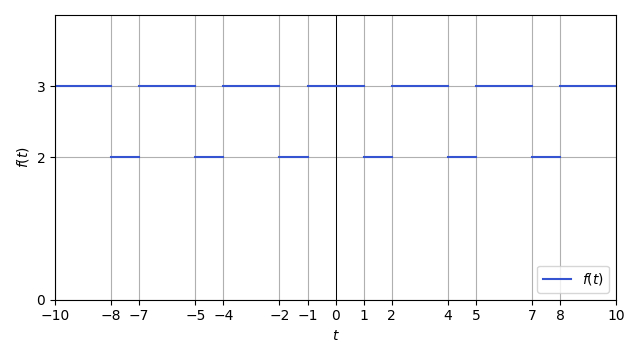
\includegraphics[width=0.7\textwidth]{square_wave/func.png}
    \caption{График функции $f(t)$}
\end{figure}\noindent
Итак, период функции $f(t)$ равен $T = 3 \ \Rightarrow\  \omega_n = \nicefrac{2\pi n}{3}$. Пришло время найти коэффициенты Фурье для этой функции --- вычислим первые три $a_n$, $b_n$ и $c_n$ ручками, а дальше за нас всё сделает машина ;)
\addsubsubsection{Считаем интегральчики...}
\NB: Т.к. перед нами кусочная функция, то нам необходимо разложить интегралы на два: один от $t_0$ до $t_1$, другой от $t_1$ до $t_2$, но при этом длина $T$ в $\omega_n$ сохраняется для обоих интегралов.\\[0.5em]
Начнём расчёты с $a_n$:
$$a_0 = \frac{2}{3}\left( \int_{4}^{5} 2\,dt + \int_{5}^{7} 3\,dt \right) = \frac{2}{3}\left( 2t\at^5_4 + 3t\at^7_5 \right) = \frac{2}{3}\left( 10 - 8 + 21 - 15\right) = \msquared{\frac{16}{3}}$$
$$a_1 = \frac{2}{3}\left( \int_{4}^{5} 2\cos\frac{2\pi t}{3}\,dt + \int_{5}^{7} 3\cos\frac{2\pi t}{3}\,dt \right) = \frac{2}{3}\left( \frac{3\sin \frac{2\pi t}{3}}{\pi}\at^5_4 + \frac{9\sin\frac{2\pi t}{3}}{2\pi}\at^7_5\right) = \frac{2}{3}\left(\frac{9\sqrt{3}}{2\pi} -\frac{3\sqrt{3}}{\pi} \right) = \msquared{\frac{\sqrt{3}}{\pi}}$$
$$a_2 = \frac{2}{3}\left( \int_{4}^{5} 2\cos\frac{4\pi t}{3}\,dt + \int_{5}^{7} 3\cos\frac{4\pi t}{3}\,dt \right) = \frac{2}{3}\left( \frac{3\sin \frac{4\pi t}{3}}{2\pi}\at^5_4 + \frac{9\sin\frac{2\pi t}{3}}{2\pi}\at^7_5\right) = \frac{2}{3}\left(\frac{3\sqrt{3}}{2\pi} -\frac{9\sqrt{3}}{4\pi} \right) = \msquared{-\frac{\sqrt{3}}{2\pi}}$$
Казалось бы, всё хорошо, но давайте найдём $a_3$ (это действительно важно!), при котором $\omega_3 = \nicefrac{2\cdot\cancel{3}\pi}{\cancel{3}} = 2\pi$:
$$a_3 = \frac{2}{3}\left( \int_{4}^{5} 2\cos2\pi t\,dt + \int_{5}^{7} 3\cos2\pi t\,dt \right) = \frac{2}{3}\left( \frac{\sin2\pi t}{\pi}\at^5_4 + \frac{3\sin2\pi t}{2\pi}\at^7_5\right) =\msquared{0}\ \ \text{ т.к. }\forall\,t,k \in \mathbb{Z}\colon\sin2k\pi t = 0$$
Становится понятно, что все коэффициенты $a_n$ при $n \divby 3$ равны нулю. Теперь найдём коэффициенты $b_n$:
$$b_1 = \frac{2}{3}\left( \int_{4}^{5} 2\sin\frac{2\pi t}{3}\,dt + \int_{5}^{7} 3\sin\frac{2\pi t}{3}\,dt \right) = -\frac{2}{3}\left( \frac{3\cos\frac{2\pi t}{3}}{\pi}\at_4^5 + \frac{9\cos \frac{2\pi t}{3}}{2\pi}\at_5^7 \right) = \msquared{0}$$
$$b_2 = \frac{2}{3}\left( \int_{4}^{5} 2\sin\frac{4\pi t}{3}\,dt + \int_{5}^{7} 3\sin\frac{4\pi t}{3}\,dt \right) = \msquared{0}\ \ \text{ т.к. косинусы вновь взаимно уничтожат друг друга.}$$
Приходим к выводу, что все коэффициенты $b_n$ равны нулю. В сущности это следует и из того, что функция чётная --- такие функции раскладываются в ряд Фурье только по косинусам. На очереди коэффициенты $c_n$:
$$c_0 = \frac{1}{3}\left( \int_{4}^{5} 2\,dt + \int_{5}^{7} 3\,dt \right) = \frac{a_0}{2} = \msquared{\frac{8}{3}}$$
\NB: Для коэффициентов $c_n$ будет использоваться свойство $\e^{2ki\pi} = 1$ $\forall k \in \mathbb{Z}$, связанное с кратностью $\cos2k\pi t = 1$ и $\sin2k\pi t = 0$.
$$c_1 = \frac{1}{3}\left( \int_{4}^{5} 2\e^{-\frac{2\pi it}{3}}\,dt + \int_{5}^{7} 3\e^{-\frac{2\pi it}{3}}\,dt \right) = \frac{i}{\pi}\left( \e^{-\frac{10\pi i}{3}}-\e^{-\frac{8\pi i}{3}} \right) + \frac{3i}{2\pi}\left( \e^{-\frac{14\pi i}{3}} - \e^{-\frac{10\pi i}{3}} \right) = \frac{i}{\pi}\left( \e^{\frac{2\pi i}{3}}-\e^{-\frac{2\pi i}{3}} \right) +$$
$$+ \frac{3i}{2\pi}\left( \e^{-\frac{2\pi i}{3}} - \e^{\frac{2\pi i}{3}} \right) = \e^{\frac{2\pi i}{3}}\left( \frac{i}{\pi} - \frac{3i}{2\pi} \right) + \e^{-\frac{2\pi i}{3}}\left( \frac{3i}{2\pi} - \frac{i}{\pi} \right) = \frac{i}{2\pi}\e^{-\frac{2\pi i}{3}}-\frac{i}{2\pi}\e^{\frac{2\pi i}{3}} = \msquared{\frac{i}{2\pi}\left( \e^{-\frac{2\pi i}{3}}-\e^{\frac{2\pi i}{3}} \right)}$$
$$c_2 = \frac{1}{3}\left( \int_{4}^{5} 2\e^{-\frac{4\pi it}{3}}\,dt + \int_{5}^{7} 3\e^{-\frac{4\pi it}{3}}\,dt \right) = \frac{i}{2\pi}\left( \e^{-\frac{20\pi i}{3}}-\e^{-\frac{16\pi i}{3}} \right) + \frac{3i}{4\pi}\left( \e^{-\frac{28\pi i}{3}} - \e^{-\frac{20\pi i}{3}} \right) = \frac{i}{2\pi}\left( \e^{-\frac{2\pi i}{3}}-\e^{\frac{2\pi i}{3}} \right) +$$
$$+ \frac{3i}{4\pi}\left( \e^{\frac{2\pi i}{3}} - \e^{-\frac{2\pi i}{3}} \right) = \e^{\frac{2\pi i}{3}} \left( \frac{3i}{4\pi} - \frac{i}{2\pi} \right) + \e^{-\frac{2\pi i}{3}} \left( \frac{i}{2\pi} - \frac{3i}{4\pi} \right) = \frac{i}{4\pi}\e^{\frac{2\pi i}{3}}-\frac{i}{4\pi}\e^{-\frac{2\pi i}{3}} = \msquared{-\frac{i}{4\pi}\left( \e^{-\frac{2\pi i}{3}} - \e^{\frac{2\pi i}{3}} \right)}$$
Хоть мы и знаем, заглядывая наперёд, что $c_3 = c_{-3} = 0$, давайте всё же проверим себя, вычислив $c_3$:
$$c_3 = \frac{1}{3}\left( \int_{4}^{5} 2\e^{-2\pi it}\,dt + \int_{5}^{7} 3\e^{-2\pi it}\,dt \right) = \frac{i}{3\pi}\left( \e^{-10\pi i} - \e^{-8\pi i} \right) + \frac{i}{2\pi}\left( \e^{-14\pi i} - \e^{-10\pi i} \right) = \frac{i}{3\pi}\left( \cancel{\e^{2\pi i}} - \cancel{\e^{2\pi i}} \right) +$$
$$+ \frac{i}{2\pi}\left( \cancel{\e^{2\pi i}} - \cancel{\e^{2\pi i}} \right) = \msquared{0}$$
\addsubsubsection{А теперь кодим!}
Напишем программу, которая вычисляет коэффициенты Фурье самостоятельно для любого $n$.
\begin{lstlisting}[language=Python, caption=Вычисление коэффициентов Фурье для кусочной функции]
from typing import Callable

import numpy as np

T = 3


def dot_product(f: Callable, g: Callable, a: float, b: float) -> np.ndarray:
    """Вычисляет скалярное произведение функций f и g на отрезке [a, b]."""
    x = np.linspace(a, b, 10000)  # Генерируем точки на отрезке [a, b]
    dx = x[1] - x[0]  # Шаг интегрирования
    return np.dot(f(x), g(x)) * dx  # Возвращаем скалярное произведение


def f(t):
    """Функция, для которой вычисляются коэффициенты Фурье."""
    # В данном случае периодическая кусочная функция
    return np.vectorize(lambda t: 2 if 0 <= (t - 1) % 3 < 1 else 3)(t)


def a(n: int, func: Callable = f, s: float = -T / 2, p: float = T) -> np.ndarray:
    """Вычисляет коэффициент a_n для функции func на отрезке (s, s + p)."""
    return 2 / p * dot_product(func, lambda t: np.cos(w(p) * n * t), s, s + p)


def b(n: int, func: Callable = f, s: float = -T / 2, p: float = T) -> np.ndarray:
    """Вычисляет коэффициент b_n для функции func на отрезке (s, s + p)."""
    return 2 / p * dot_product(func, lambda t: np.sin(w(p) * n * t), s, s + p)


def c(n, func: Callable = f, s: float = -T / 2, p: float = T) -> np.ndarray:
    """Вычисляет коэффициент c_n для функции func на отрезке (s, s + p)."""
    return 1 / p * dot_product(func, lambda t: np.exp(-1j * w(p) * n * t), s, s + p)


def fourier_coefficients(n: int):
    """Вычисляет коэффициенты Фурье a_n, b_n и c_n для функции f с периодом T."""
    return a(n).round(3), b(n).round(3), c(n).round(3), c(-n).round(3)


# Задаем период функции и порядковый номер коэффициента
print('Оставьте поле ввода пустым, и программа выведет первые 6 коэффициентов Фурье, начиная с 0.')
coef_num = int(data) if (data := input('Введите порядковый номер коэффициента: ')) else None
w = lambda period: 2 * np.pi / period

# Выводим коэффициенты Фурье (либо первые 6, либо введенный пользователем)
for n in range(coef_num or 0, (coef_num or 5) + 1):
    a_n, b_n, c_n, c_mn = fourier_coefficients(n)
    print(f'a_{n} = {a_n},\tb_{n} = {b_n},\tc_{n} = {c_n}  c_{-n} = {c_mn}')    
\end{lstlisting}
Итак, программа выведет нам первые шесть коэффициентов Фурье для функции $f(t)$, среди которых есть и необходимые по заданию $a_3$, $b_3$ и $c_3$ --- хотя они всё равно равны нулю, чего тут смотреть :)
\begin{lstlisting}[caption=Вывод программы]
a_0 = 5.334,    b_0 = 0.0,      c_0 = (2.667+0j)  c_0 = (2.667+0j)
a_1 = 0.551,    b_1 = 0.0,      c_1 = (0.275-0j)  c_-1 = (0.275+0j)
a_2 = -0.275,   b_2 = -0.0,     c_2 = (-0.138+0j)  c_-2 = (-0.138-0j)
a_3 = -0.0,     b_3 = 0.0,      c_3 = (-0-0j)  c_-3 = (-0+0j)
a_4 = 0.138,    b_4 = 0.0,      c_4 = (0.069-0j)  c_-4 = (0.069+0j)
a_5 = -0.111,   b_5 = -0.0,     c_5 = (-0.055+0j)  c_-5 = (-0.055-0j)
\end{lstlisting}\newpage
\addsubsubsection{Созерцаем плоды трудов!}
Воспользуемся этими коэффициентами для построения графиков тригонометрического $F_n$ и экспоненциального $G_n$ рядов Фурье для функции $f(t)$:
\begin{figure}[H]
    \begin{minipage}{0.5\textwidth}
        \centering 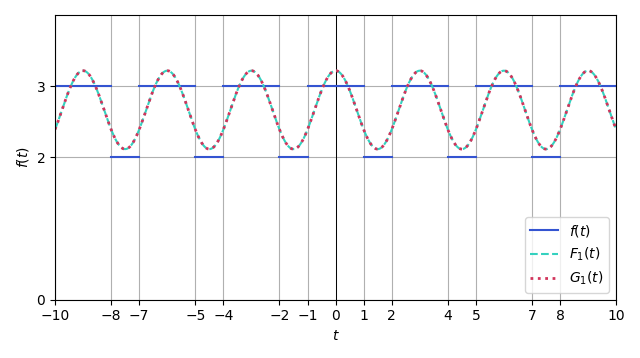
\includegraphics[width=\textwidth]{square_wave/1.png}
        \caption{$n = 1$}
    \end{minipage}\hfill
    \begin{minipage}{0.5\textwidth}
        \centering 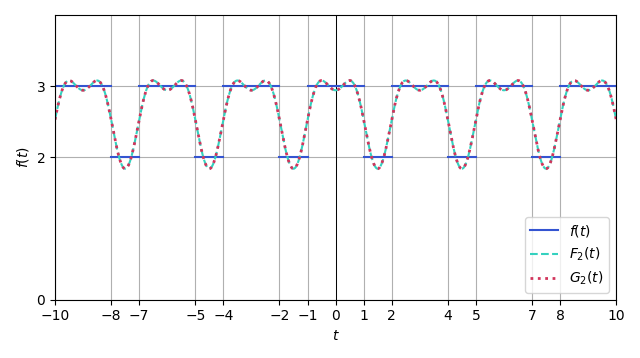
\includegraphics[width=\textwidth]{square_wave/2.png}
        \caption{$n = 2$}
    \end{minipage}\\[1em]
    \begin{minipage}{0.5\textwidth}
        \centering 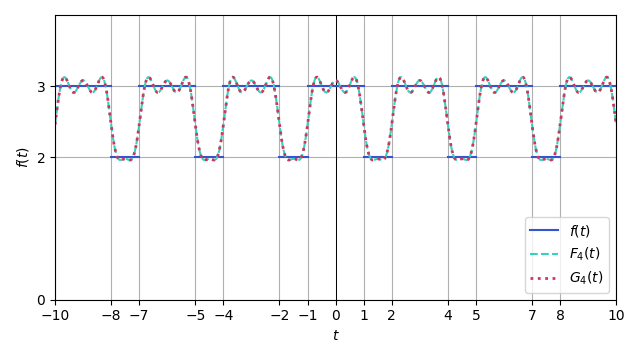
\includegraphics[width=\textwidth]{square_wave/4.png}
        \caption{$n = 4$}
    \end{minipage}\hfill
    \begin{minipage}{0.5\textwidth}
        \centering 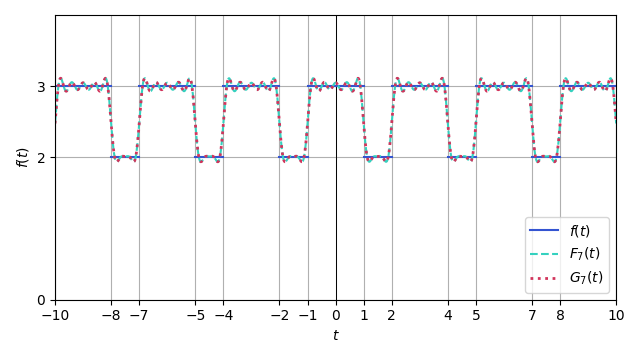
\includegraphics[width=\textwidth]{square_wave/7.png}
        \caption{$n = 7$}
    \end{minipage}\\[1em]
    \begin{minipage}{0.5\textwidth}
        \centering 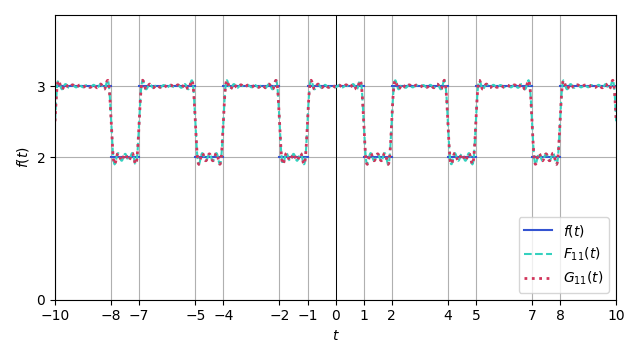
\includegraphics[width=\textwidth]{square_wave/11.png}
        \caption{$n = 11$}
    \end{minipage}
    \begin{minipage}{0.5\textwidth}
        \centering 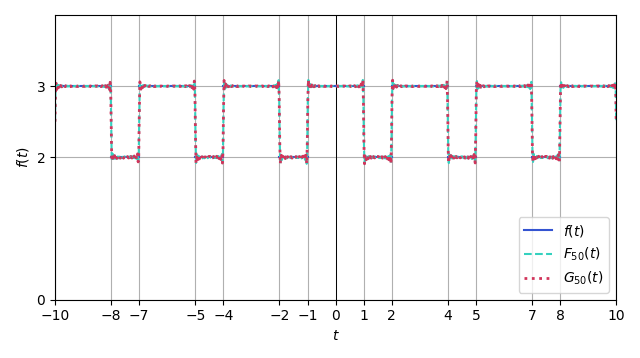
\includegraphics[width=\textwidth]{square_wave/50.png}
        \caption{$n = 50$}
    \end{minipage}
\end{figure}\noindent
Как мы видим, ряды Фурье $F_n(t)$ и $G_n(t)$:
\begin{itemize}
    \item во-первых, совпадают;
    \item во-вторых, шедевральны;
    \item в-третьих, вполне неплохо аппроксимируют функцию $f(t)$ уже при $n = 7$;
    \item и, наконец, разница, без учёта эффекта Гиббса практически незаметна при $n = 50$.
\end{itemize}
Чтобы убедиться в том, что при $n = 50$ ряд Фурье действительно хорошо приближается к функции $f(t)$, проверим равенство Парсеваля при этом же количестве коэффициентов и при $n = 1$ --- так мы увидим разницу.
\begin{minipage}{0.48\textwidth}
\begin{lstlisting}[caption={Равенство Парасеваля при $n=1$}]
Parseval deviation:
| |f|^2 - sum(|a_i|^2 + |b_i|^2) | = 1.35317
| |f|^2 - sum(|c_i|^2) |           = 1.35317
\end{lstlisting}
\end{minipage}\hfill
\begin{minipage}{0.49\textwidth}
\begin{lstlisting}[caption={Равенство Парасеваля при $n=50$}, numbers=none]
Parseval deviation:
| |f|^2 - sum(|a_i|^2 + |b_i|^2) | = 0.01964
| |f|^2 - sum(|c_i|^2) |           = 0.01964
\end{lstlisting}
\end{minipage}
Мы наблюдаем, что отклонение в равенстве Парсеваля с увеличением количества коэффициентов стремится к нулю. Это означает, что ряд Фурье действительно приближается к функции $f(t)$ всё лучше и лучше.\\[0.5em]

\addsubsection{Время чётных функций!}
Теперь рассмотрим чётную периодическую функцию $f(x) = |2\sin x|$ на отрезке $[0, \pi]$ --- брать чистый синус со стандартным промежутком не интересно, а так будет хоть какое-то разнообразие. И, конечно, построим график этой функции.
\begin{figure}[H]
    \centering 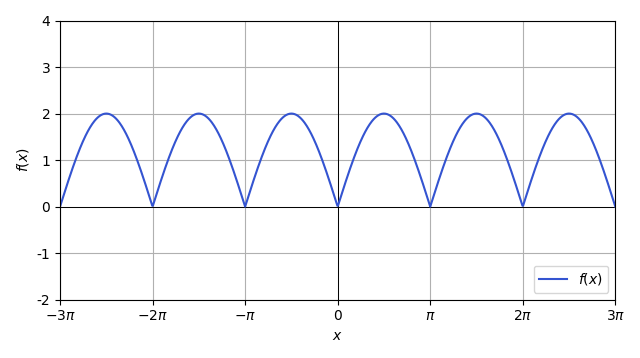
\includegraphics[width=0.7\textwidth]{even_func/func.png}
    \caption{График функции $f(x)$}
\end{figure}\noindent
Период функции $f(x)$ равен $T = \pi \ \Rightarrow\  \omega_n = 2n$. И снова настало время найти коэффициенты Фурье теперь для этой функции, но мы стали умными и у нас есть код, поэтому пускай за нас всё делает машина ;)\\[0.5em]
Однако же не будет лишним привести формулу для вычисления коэффициентов. Для чётной функции $f(x)$ коэффициенты $b_n$ равны нулю и ряд Фурье строится по косинусам. Таким образом, коэффициенты $a_n$ и $c_n$ в общем виде вычисляются следующим образом:
$$a_n = \frac{2}{\pi}\int_{0}^{\pi} |2\sin x|\cos 2nx\,dx\qquad c_n = \frac{1}{\pi}\int_{0}^{\pi}|2\sin x|\e^{-2inx}\,dx$$
\newpage
\addsubsubsection{Снова немножко кодим...}
Изменим программу, которая вычисляет коэффициенты Фурье самостоятельно для любого $n$, под нашу функцию.
\begin{lstlisting}[language=Python, caption={Вычисление коэффициентов Фурье для функции $|2\sin x|$}]
...

def f(x):
    """Функция, для которой вычисляются коэффициенты Фурье."""
    return np.vectorize(lambda x: 2*np.abs(np.sin(x)))(x)

...   
\end{lstlisting}
Программа вновь выводит нам первые шесть коэффициентов Фурье, среди которых есть и необходимые по заданию $a_3$, $b_3$ и $c_3$:
\begin{lstlisting}[caption=Вывод программы]
a_0 = 2.547,    b_0 = 0.0,      c_0 = (1.273+0j)  c_0 = (1.273+0j)
a_1 = -0.849,   b_1 = 0.0,      c_1 = (-0.425+0j)  c_-1 = (-0.425-0j)
a_2 = -0.169,   b_2 = -0.0,     c_2 = (-0.085+0j)  c_-2 = (-0.085-0j)
a_3 = -0.073,   b_3 = -0.0,     c_3 = (-0.037-0j)  c_-3 = (-0.037+0j)
a_4 = -0.04,    b_4 = 0.0,      c_4 = (-0.02-0j)  c_-4 = (-0.02+0j)
a_5 = -0.026,   b_5 = -0.0,     c_5 = (-0.013-0j)  c_-5 = (-0.013+0j)
\end{lstlisting}
Убеждаемся, что, действительно, коэффициенты $b_n$ равны нулю.
\addsubsubsection{Рисуем графики!}
Воспользуемся этими коэффициентами для построения графиков тригонометрического $F_n$ и экспоненциального $G_n$ рядов Фурье для функции $f(x)$:
\begin{figure}[H]
    \begin{minipage}{0.5\textwidth}
        \centering 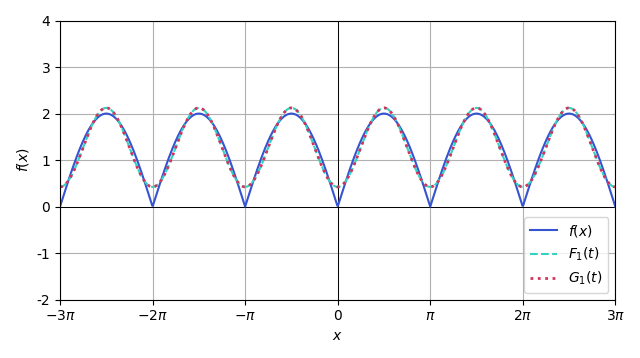
\includegraphics[width=\textwidth]{even_func/1.png}
        \caption{$n = 1$}
    \end{minipage}\hfill
    \begin{minipage}{0.5\textwidth}
        \centering 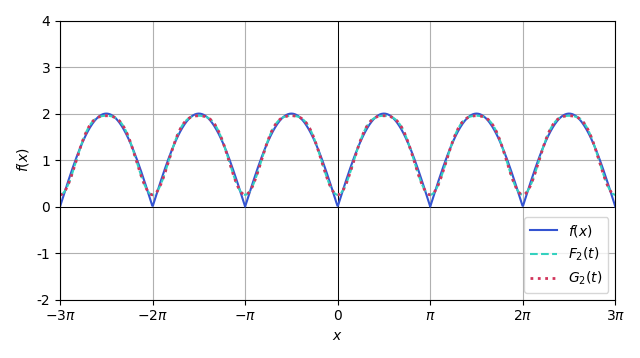
\includegraphics[width=\textwidth]{even_func/2.png}
        \caption{$n = 2$}
    \end{minipage}\\[2em]
    \begin{minipage}{0.5\textwidth}
        \centering 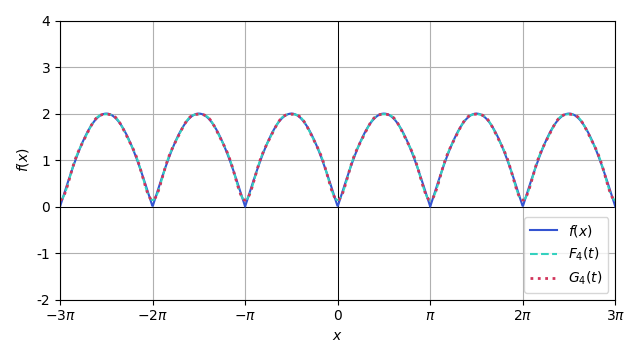
\includegraphics[width=\textwidth]{even_func/4.png}
        \caption{$n = 4$}
    \end{minipage}\hfill
    \begin{minipage}{0.5\textwidth}
        \centering 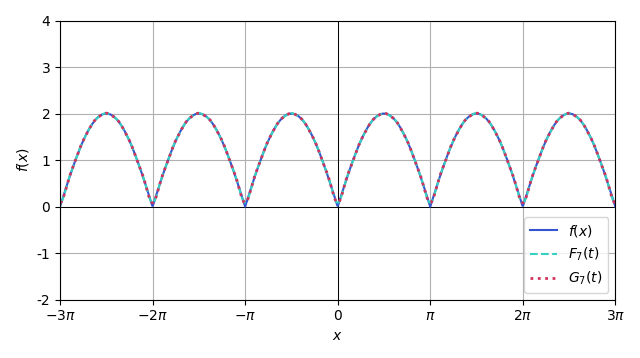
\includegraphics[width=\textwidth]{even_func/7.png}
        \caption{$n = 7$}
    \end{minipage}
\end{figure}
\begin{figure}[H]
    \begin{minipage}{0.5\textwidth}
        \centering 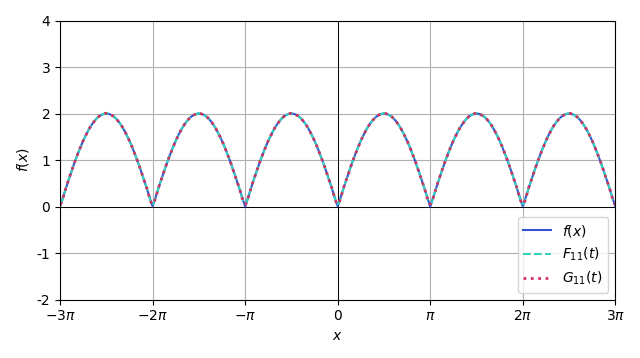
\includegraphics[width=\textwidth]{even_func/11.png}
        \caption{$n = 11$}
    \end{minipage}
    \begin{minipage}{0.5\textwidth}
        \centering 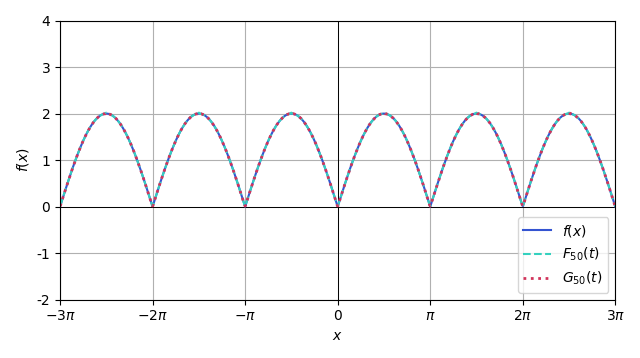
\includegraphics[width=\textwidth]{even_func/50.png}
        \caption{$n = 50$}
    \end{minipage}
\end{figure}\noindent
И вновь графики рядов Фурье $F_n(x)$ и $G_n(x)$ совпадают и хорошо аппроксимируют функцию $f(x)$. Ввиду простоты функции $f(x)$, разница между графиками рядов Фурье и функции практически незаметна даже при $n = 4$. Более того, не наблюдается эффекта Гиббса, т.к. у функции нет разрывов.\\[0.5em]
Чтобы убедиться в том, что при $n = 50$ ряд Фурье действительно аппроксимирует функцию $f(x)$ довольно точно, проверим равенство Парсеваля при этом же количестве коэффициентов и при $n = 1$ --- так мы увидим разницу.
\begin{minipage}{0.48\textwidth}
\begin{lstlisting}[caption={Равенство Парасеваля при $n=1$}]
Parseval deviation:
| |f|^2 - sum(|a_i|^2 + |b_i|^2) | = 2.38045
| |f|^2 - sum(|c_i|^2) |           = 2.38045
\end{lstlisting}
\end{minipage}\hfill
\begin{minipage}{0.49\textwidth}
\begin{lstlisting}[caption={Равенство Парасеваля при $n=50$}, numbers=none]
Parseval deviation:
| |f|^2 - sum(|a_i|^2 + |b_i|^2) | = 0.00003
| |f|^2 - sum(|c_i|^2) |           = 0.00003
\end{lstlisting}
\end{minipage}
Мы наблюдаем, что отклонение в равенстве Парсеваля с увеличением количества коэффициентов стремится к нулю. Это означает, что ряд Фурье действительно приближается к функции $f(x)$ всё лучше и лучше.\\[0.5em]

\addsubsection{Ты чего такой нечётный?}
Настал черёд нечётной периодической функцию $f(x) = \left( (x - 2) \bmod 4 - 2 \right)^3$ на отрезке $[-2, 2]$. Кто бы мог подумать, что для периодичности кубического корня нужно так усложнять аргумент внутри? Но это всё лирика, поэтому давайте уже строить график функции.
\begin{figure}[H]
    \centering 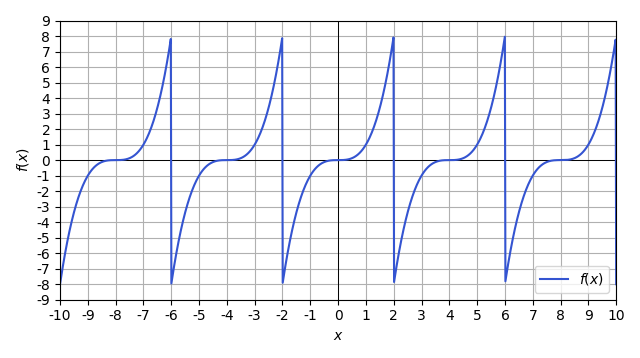
\includegraphics[width=0.831\textwidth]{odd_func/func.png}
    \caption{График функции $f(x)$}
\end{figure}\noindent
Период функции $f(x)$ равен $T = 4 \ \Rightarrow\  \omega_n = \nicefrac{n\pi}{2}$. Вновь найдём коэффициенты Фурье для функции с помощью уже написанной нами ранее программы, но перед этим посмотрим на интегралы. Для нечётной функции $f(x)$ коэффициенты $a_n$ равны нулю и ряд Фурье строится по синусам. Таким образом, коэффициенты $b_n$ и $c_n$ в общем виде вычисляются следующим образом:
$$b_n = \frac{1}{2}\int_{-2}^{2} \left( (x - 2) \bmod 4 - 2 \right)^3\sin \frac{n\pi x}{2}\,dx\qquad c_n = \frac{1}{4}\int_{-2}^{2}\left( (x - 2) \bmod 4 - 2 \right)^3\e^{\nicefrac{-in\pi x}{2}}\,dx$$
\addsubsubsection{Опять кодим одну строчку}
Изменим программу, которая вычисляет коэффициенты Фурье самостоятельно для любого $n$, под нашу функцию.
\begin{lstlisting}[language=Python, caption={Вычисление коэффициентов Фурье для функции $f(x)$}]
...

def f(x):
    """Функция, для которой вычисляются коэффициенты Фурье."""
    return np.vectorize(lambda x: ((x - 2) % 4 - 2) ** 3)(x)

...   
\end{lstlisting}
Программа вновь выводит нам первые шесть коэффициентов Фурье, среди которых есть и необходимые по заданию $a_3$, $b_3$ и $c_3$:
\begin{lstlisting}[caption=Вывод программы]
a_0 = -0.0,   b_0 = 0.0,      c_0 = (-0+0j)  c_0 = (-0.002+0j)
a_1 = 0.0,    b_1 = 1.997,    c_1 = (0-0.998j)  c_-1 = (0.002+0.998j)
a_2 = -0.0,   b_2 = -2.159,   c_2 = (-0+1.08j)  c_-2 = (-0.002-1.08j)
a_3 = 0.0,    b_3 = 1.583,    c_3 = (0.002-0.791j)  c_-3 = (0.002+0.791j)
a_4 = -0.0,   b_4 = -1.225,   c_4 = (-0+0.612j)  c_-4 = (-0.002-0.612j)
a_5 = 0.0,    b_5 = 0.994,    c_5 = (0-0.497j)  c_-5 = (0.002+0.497j)
\end{lstlisting}
Убеждаемся в том, что, действительно, коэффициенты $a_n$ равны нулю.
\addsubsubsection{И снова любуемся на рисунки!}
Воспользуемся этими коэффициентами для построения графиков тригонометрического $F_n$ и экспоненциального $G_n$ рядов Фурье для функции $f(x)$:
\begin{figure}[H]
    \begin{minipage}{0.5\textwidth}
        \centering 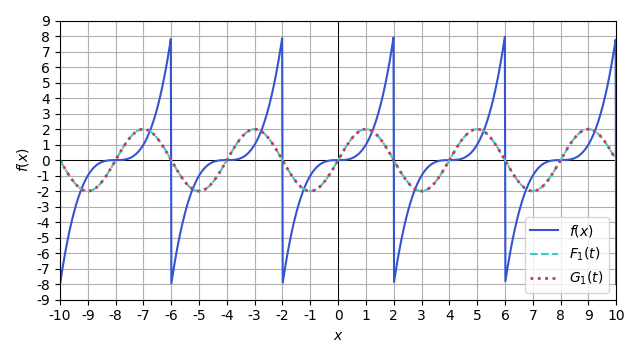
\includegraphics[width=\textwidth]{odd_func/1.png}
        \caption{$n = 1$}
    \end{minipage}\hfill
    \begin{minipage}{0.5\textwidth}
        \centering 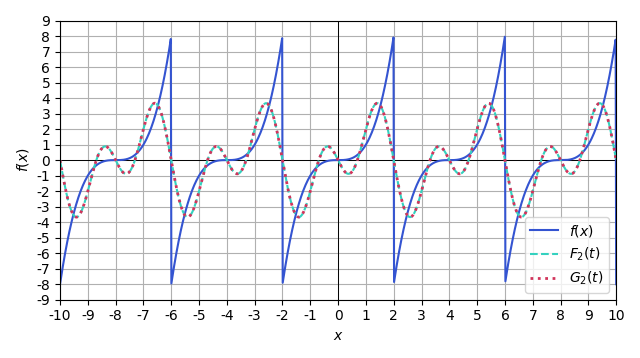
\includegraphics[width=\textwidth]{odd_func/2.png}
        \caption{$n = 2$}
    \end{minipage}
\end{figure}
\begin{figure}[H]
    \begin{minipage}{0.5\textwidth}
        \centering 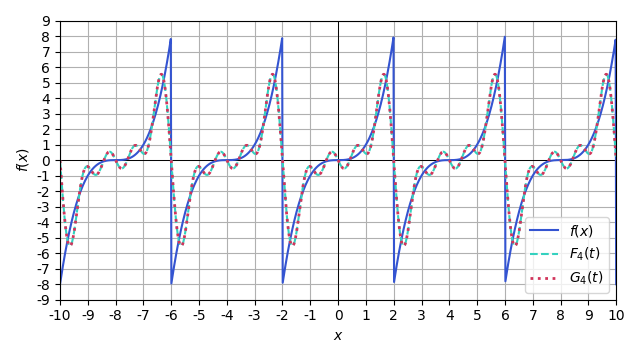
\includegraphics[width=\textwidth]{odd_func/4.png}
        \caption{$n = 4$}
    \end{minipage}\hfill
    \begin{minipage}{0.5\textwidth}
        \centering 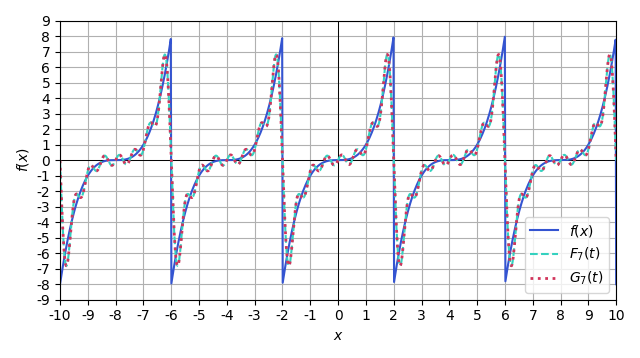
\includegraphics[width=\textwidth]{odd_func/7.png}
        \caption{$n = 7$}
    \end{minipage}\\[2em]
    \begin{minipage}{0.5\textwidth}
        \centering 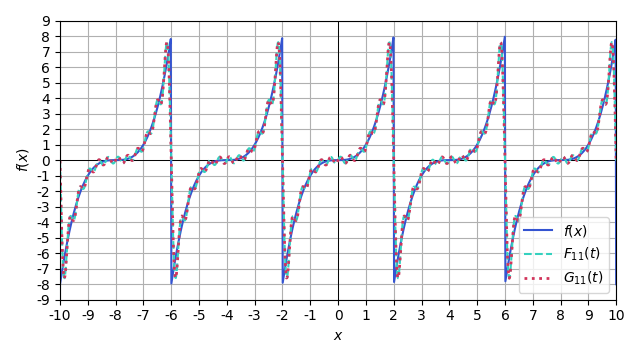
\includegraphics[width=\textwidth]{odd_func/11.png}
        \caption{$n = 11$}
    \end{minipage}
    \begin{minipage}{0.5\textwidth}
        \centering 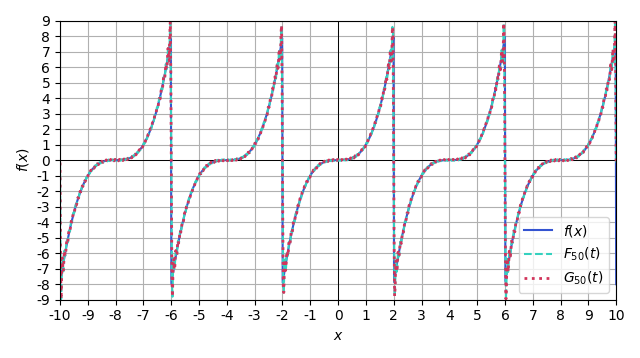
\includegraphics[width=\textwidth]{odd_func/50.png}
        \caption{$n = 50$}
    \end{minipage}
\end{figure}\noindent
Графики рядов Фурье $F_n(x)$ и $G_n(x)$ совпадают и хорошо приближаются к функции $f(x)$ при $n > 7$. Также не наблюдается эффекта Гиббса, т.к. у функции имеется разрыв только по вертикальной асимптоте.\\[0.5em]
Чтобы убедиться в том, что при $n = 50$ ряд Фурье аппроксимирует функцию $f(x)$ очень точно, проверим равенство Парсеваля при этом же количестве коэффициентов и при $n = 1$ --- так мы увидим разницу.\\
\begin{minipage}{0.48\textwidth}
\begin{lstlisting}[caption={Равенство Парасеваля при $n=1$}]
Parseval deviation:
| |f|^2 - sum(|a_i|^2 + |b_i|^2) | = 23.80626
| |f|^2 - sum(|c_i|^2) |           = 23.80626
\end{lstlisting}
\end{minipage}\hfill
\begin{minipage}{0.49\textwidth}
\begin{lstlisting}[caption={Равенство Парасеваля при $n=50$}, numbers=none]
Parseval deviation:
| |f|^2 - sum(|a_i|^2 + |b_i|^2) | = 0.00068
| |f|^2 - sum(|c_i|^2) |           = 0.00068
\end{lstlisting}
\end{minipage}
Мы  наблюдаем, что отклонение в равенстве Парсеваля с увеличением количества коэффициентов стремится к нулю. Это означает, что ряд Фурье действительно представляет функцию $f(x)$ всё лучше и лучше.\newpage
\addsubsection{Ты вообще с какого района, чушпан?}
Наконец, рассмотрим периодическую функцию, являющуюся ни чётной, ни нечётной --- в студии\break $f(x) = \left(\nicefrac{x}{\pi} \bmod 2\right)^2$ на отрезке $[0, 2\pi]$ --- а вот это будет интересно... И, по традиции, построим график этой функции.
\begin{figure}[H]
    \centering 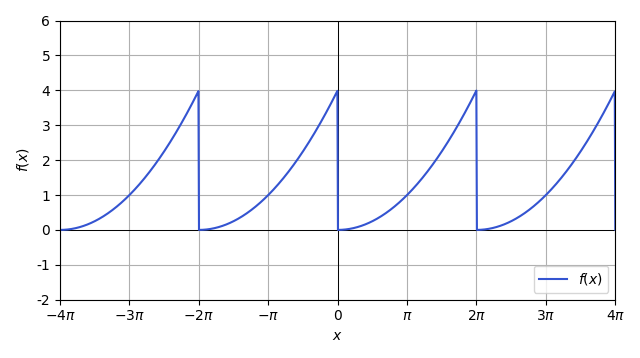
\includegraphics[width=0.7\textwidth]{periodic_func/func.png}
    \caption{График функции $f(x)$}
\end{figure}\noindent
Период функции $f(x)$ равен $T = 2\pi \ \Rightarrow\  \omega_n = n$. Найдём коэффициенты Фурье для функции с помощью уже написанной программы, но перед этим взглянем на то, как вычисляются коэффициенты $a_n$, $b_n$ и $c_n$ в общем виде:
$$a_n = \frac{1}{\pi}\int_{0}^{2\pi} \left(\frac{x}{\pi} \bmod 2\right)^2\sin nx\,dx\qquad b_n = \frac{1}{\pi}\int_{0}^{2\pi} \left(\frac{x}{\pi} \bmod 2\right)^2\cos nx\,dx\qquad c_n = \frac{1}{2\pi}\int_{0}^{2\pi}\left(\frac{x}{\pi} \bmod 2\right)^2\e^{-inx}\,dx$$
\addsubsubsection{Немножко помучаем машину...}
Изменим в программе функцию, для которой вычисляются коэффициенты Фурье:
\begin{lstlisting}[language=Python, caption={Вычисление коэффициентов Фурье для функции $f(x)$}]
...

def f(x):
    """Функция, для которой вычисляются коэффициенты Фурье."""
    return np.vectorize(lambda x: ((x / np.pi) % 2) ** 2)(x)

...   
\end{lstlisting}
Программа вновь выводит нам первые шесть коэффициентов Фурье, среди которых есть и необходимые по заданию $a_3$, $b_3$ и $c_3$:
\begin{lstlisting}[caption=Вывод программы]
a_0 = 2.997,    b_0 = 0.0,      c_0 = (1.499+0j)      c_0 = (1.499+0j)
a_1 = 0.352,    b_1 = -1.736,   c_1 = (0.176+0.868j)  c_-1 = (0.176-0.868j)
a_2 = 0.041,    b_2 = -0.405,   c_2 = (0.021+0.203j)  c_-2 = (0.021-0.203j)
a_3 = 0.039,    b_3 = -0.579,   c_3 = (0.019+0.289j)  c_-3 = (0.019-0.289j)
a_4 = 0.01,     b_4 = -0.203,   c_4 = (0.005+0.101j)  c_-4 = (0.005-0.101j)
a_5 = 0.014,    b_5 = -0.347,   c_5 = (0.007+0.174j)  c_-5 = (0.007-0.174j)
\end{lstlisting}
\addsubsubsection{И что же получилось на графиках?}
Воспользуемся этими коэффициентами для построения графиков тригонометрического $F_n$ и экспоненциального $G_n$ рядов Фурье для функции $f(x)$:
\begin{figure}[H]
    \begin{minipage}{0.5\textwidth}
        \centering 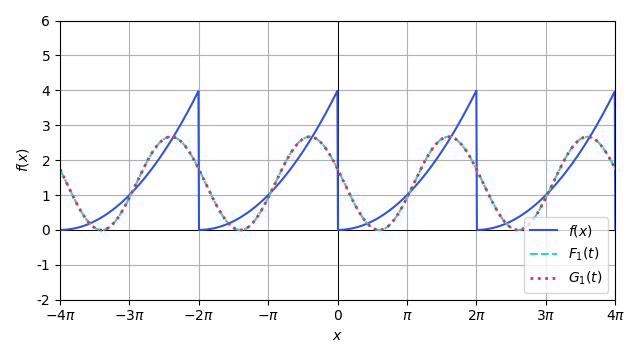
\includegraphics[width=\textwidth]{periodic_func/1.png}
        \caption{$n = 1$}
    \end{minipage}\hfill
    \begin{minipage}{0.5\textwidth}
        \centering 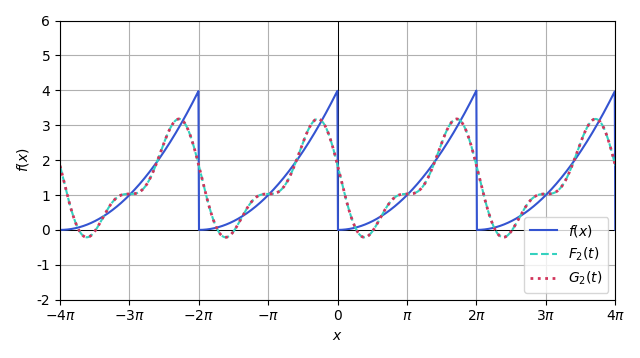
\includegraphics[width=\textwidth]{periodic_func/2.png}
        \caption{$n = 2$}
    \end{minipage}\\[2em]
    \begin{minipage}{0.5\textwidth}
        \centering 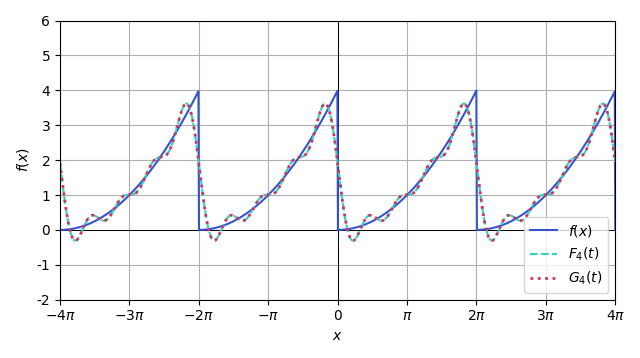
\includegraphics[width=\textwidth]{periodic_func/4.png}
        \caption{$n = 4$}
    \end{minipage}\hfill
    \begin{minipage}{0.5\textwidth}
        \centering 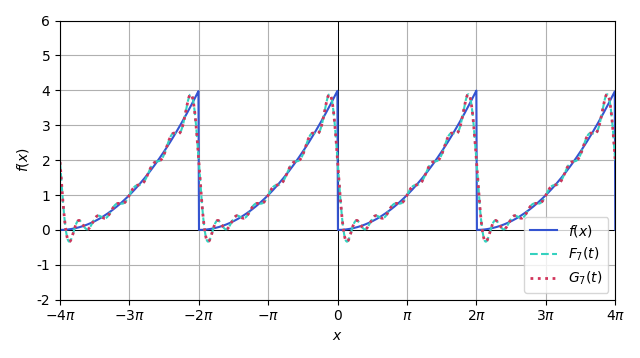
\includegraphics[width=\textwidth]{periodic_func/7.png}
        \caption{$n = 7$}
    \end{minipage}\\[2em]
    \begin{minipage}{0.5\textwidth}
        \centering 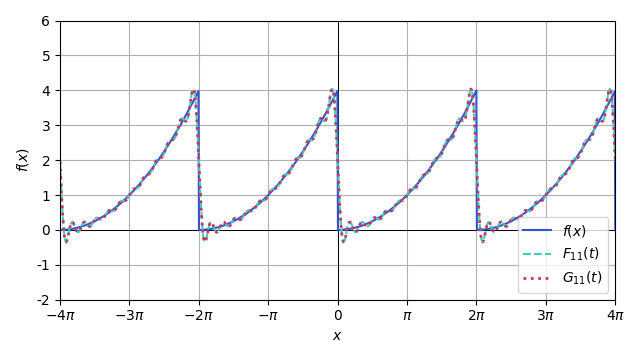
\includegraphics[width=\textwidth]{periodic_func/11.png}
        \caption{$n = 11$}
    \end{minipage}\hfill
    \begin{minipage}{0.5\textwidth}
        \centering 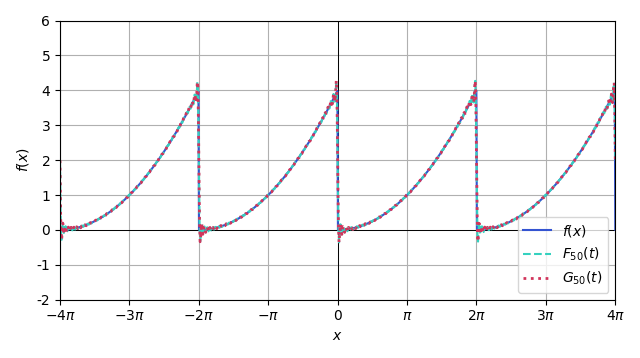
\includegraphics[width=\textwidth]{periodic_func/50.png}
        \caption{$n = 50$}
    \end{minipage}
\end{figure}\noindent
Графики рядов Фурье $F_n(x)$ и $G_n(x)$ совпадают и хорошо приближаются к функции $f(x)$ при $n > 7$ без учёта эффекта Гиббса, т.к. у функции имеется разрыв под углом.\newpage\noindent
Чтобы убедиться в том, что при $n = 50$ ряд Фурье аппроксимирует функцию $f(x)$ очень точно, проверим равенство Парсеваля при этом же количестве коэффициентов и при $n = 1$ --- так мы увидим разницу.\\
\begin{minipage}{0.48\textwidth}
\begin{lstlisting}[caption={Равенство Парасеваля при $n=1$}]
Parseval deviation:
| |f|^2 - sum(|a_i|^2 + |b_i|^2) | = 3.32656
| |f|^2 - sum(|c_i|^2) |           = 3.32656
\end{lstlisting}
\end{minipage}\hfill
\begin{minipage}{0.49\textwidth}
\begin{lstlisting}[caption={Равенство Парасеваля при $n=50$}, numbers=none]
Parseval deviation:
| |f|^2 - sum(|a_i|^2 + |b_i|^2) | = 0.10021
| |f|^2 - sum(|c_i|^2) |           = 0.10021
\end{lstlisting}
\end{minipage}
Мы наблюдаем, что отклонение в равенстве Парсеваля с увеличением количества коэффициентов стремится к нулю. Это означает, что ряд Фурье действительно аппроксимирует функцию $f(x)$ всё лучше и лучше.\\[0.5em]

\addsection{Задание №2. Комплéксная функция vs. мозг читателя}
Начнём новое задание, как и предыдущее, с небольшой теоретической справки. В прошлом задании мы говорили о представлении тригонометрического ряда Фурье с помощью $\e^{ix}$ --- это форма ряда называется \textbf{комплексным рядом Фурье}. Давайте пройдём через преобразования, которые приведут нас от коэффициентов тригонометрического ряда $a_n$ и $b_n$ к коэффициентам комплексного ряда $c_n$. Для этого воспользуемся формулами Эйлера:
$$\cos x = \frac{\e^{ix} + \e^{-ix}}{2}\qquad\sin x = \frac{\e^{ix} - \e^{-ix}}{2i}$$
И вот как будет выглядеть такое преобразование:
$$a\cos\omega t + b\sin\omega t = a\left( \frac{\e^{i\omega t} + \e^{-i\omega t}}{2} \right) + b\left( \frac{\e^{i\omega t} - \e^{-i\omega t}}{2i} \right) = \frac{a}{2}\bigg( \e^{i\omega t} + \e^{-i\omega t} \bigg) - \frac{ib}{2}\bigg( \e^{i\omega t} - \e^{-i\omega t} \bigg) =$$
$$= \frac{a - ib}{2}\e^{i\omega t}+\frac{a+ib}{2}\e^{-i\omega t} = c\e^{i\omega t} + \bar{c}\e^{-i\omega t}$$
Отсюда и выясняется причина, по которой комплексный ряд Фурье раскладывается в обе стороны от нуля --- одна пара $\left( a_n, b_n \right)$ дают два коэффициента $\left( c_n, c_{-n} \right)$, которые двигаются в противофазе. И поэтому в предыдущем задании для вещественных функций мы также рассматривали ряд $G_n$.\\[0.5em]
Говоря о комплексных функциях, $f(t)$ подобна таковой, и поэтому представляется \underline{только} в виде комплексного ряда Фурье, который выглядит следующим образом:
$$f(t) = \sum_{n=-\infty}^{\infty}c_n\e^{i\omega_nt}\text{, где }\omega_n = \frac{2\pi n}{T}$$
\begin{center}
    \line(1,0){300}
\end{center}
Зададим $R = 2$ и $T = 8\ \Rightarrow\ \omega = \nicefrac{\pi n}{4}$. И получим по заданию следующую комплекснозначную функцию, заданную параметрическим образом:
$$\text{Re}\,f(t) = \begin{cases}
    2, & t \in [-1, 1),\\
    -2t+4, & t \in [1, 3),\\
    -2, & t \in [3, 5),\\
    2t-12, & t \in [5, 7),\\
\end{cases}\qquad\text{Im}\,f(t) = \begin{cases}
    2t, & t \in [-1, 1),\\
    2, & t \in [1, 3),\\
    -2t+8, & t \in [3, 5),\\
    -2, & t \in [5, 7).\\
\end{cases}$$
\newpage\noindent
График функции $f(t)$ обозначим на комплексной плоскости:
\begin{figure}[H]
    \centering 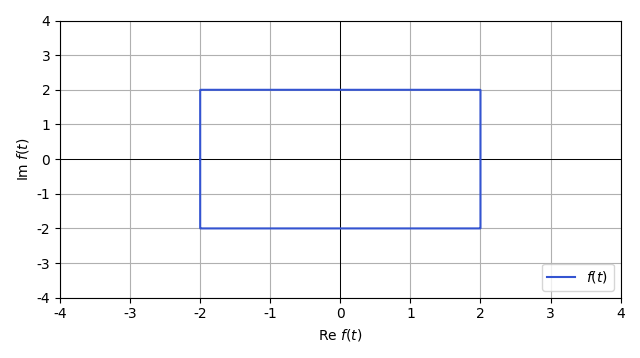
\includegraphics[width=0.7\textwidth]{parametric_func/func.png}
    \caption{График функции $f(t)$}
\end{figure}\noindent
Получаем вот такой скромненький квадратик на комплексной плоскости --- он пока одинок, но скоро обрастёт интересными подробностями ;) 
\addsubsection{Самое скучное --- вы не разучились считать интегральчики?}
Теперь найдём коэффициенты Фурье $c_n$ для этой функции, которые в общем виде вычисляются так:
$$c_n = \frac{1}{8}\int_{-1}^{7}f(t)e^{-i\frac{\pi n}{4}t}\,dt = \frac{1}{8}\left( \int_{-1}^{1} \left( 2 + 2ti \right)e^{-i\frac{\pi n}{4}t}\,dt + \int_{1}^{3}\left( -2t + 4 + 2i \right)e^{-i\frac{\pi n}{4}t}\,dt +  \right.$$$$\left. + \int_{3}^{5}\left( -2 + 8i - 2ti \right)e^{-i\frac{\pi n}{4}t}\,dt + \int_{5}^{7}\left( 2t - 12 -2i \right)e^{-i\frac{\pi n}{4}t}\,dt\right)$$
И эту громадину придётся вычислять? Конечно, да! Вычислим вручную $c_0$, $c_1$, $c_2$:
$$c_0 = \int_{-1}^{1} \frac{\left( 2 + 2ti \right)}{8}\,dt + \int_{1}^{3}\frac{\left( -2t + 4 + 2i \right)}{8}\,dt + \int_{3}^{5}\frac{\left( -2 + 8i - 2ti \right)}{8}\,dt + \int_{5}^{8}\frac{\left( 2t - 12 -2i \right)}{8}\,dt = \frac{1}{8}\left( \cancel{4} + \bcancel{4i} -\cancel{4}  -\bcancel{4i} \right) = 0$$
$$c_1 = \int_{-1}^{1} \frac{\left( 2 + 2ti \right)}{8}e^{-i\frac{\pi}{4}t}\,dt + \int_{1}^{3}\frac{\left( -2t + 4 + 2i \right)}{8}e^{-i\frac{\pi}{4}t}\,dt + \int_{3}^{5}\frac{\left( -2 + 8i - 2ti \right)}{8}e^{-i\frac{\pi}{4}t}\,dt + \int_{5}^{8}\frac{\left( 2t - 12 -2i \right)}{8}e^{-i\frac{\pi}{4}t}\,dt = $$$$= \frac{1}{8}\left( 4\cdot\frac{32\sqrt{2}}{\pi^2} \right) = \frac{16\sqrt{2}}{\pi^2}$$
$$c_2 = \int_{-1}^{1} \frac{\left( 2 + 2ti \right)}{8}e^{-i\frac{\pi}{2}t}\,dt + \int_{1}^{3}\frac{\left( -2t + 4 + 2i \right)}{8}e^{-i\frac{\pi}{2}t}\,dt + \int_{3}^{5}\frac{\left( -2 + 8i - 2ti \right)}{8}e^{-i\frac{\pi}{2}t}\,dt + \int_{5}^{7}\frac{\left( 2t - 12 -2i \right)}{8}e^{-i\frac{\pi}{2}t}\,dt =$$$$= \frac{1}{8}\left( \cancel{\frac{8}{\pi} + \frac{16}{\pi^2}} - \bcancel{\frac{8i}{\pi} - \frac{16i}{\pi^2}} - \cancel{\frac{8}{\pi} - \frac{16}{\pi^2}} + \bcancel{\frac{8i}{\pi} + \frac{16i}{\pi^2}}\right) = 0$$
Что необычно, коэффициент $c_0$ равен нулю, хотя на комплексной плоскости хорошо видно, что функция приподнята на графике --- это из-за того, что мы рассматриваем не оси XOY, а комплексную плоскость.
\addsubsection{Самое приятное --- код всё сделает за нас}
Воспользуемся программой, которая вычисляет коэффициенты Фурье самостоятельно для любого $n$, чтобы найти требуемый в задании коэффициент $c_3$ для функции $f(t)$. Программа уже написана, поэтому мы просто вставим в неё нашу функцию и запустим её, чтобы получить коэффициенты:
\begin{lstlisting}[language=Python, caption={Вычисление коэффициентов Фурье для функции $f(t)$}]
...

def f(x):
    """Функция, для которой вычисляются коэффициенты Фурье."""
    def create_parametric_func(R, T):
        """Возвращает параметрическую функцию с заданными R и T."""
    
        def pfunc_instance(t):
            """Чистый экземпляр параметрической функции."""
            t = (t + T / 8) % T - T / 8
            if -T / 8 <= t < T / 8:
                real = R
            elif T / 8 <= t < 3 * T / 8:
                real = 2 * R - 8 * R * t / T
            elif 3 * T / 8 <= t < 5 * T / 8:
                real = -R
            elif 5 * T / 8 <= t <= 7 * T / 8:
                real = -6 * R + 8 * R * t / T

            if -T / 8 <= t < T / 8:
                imag = 8 * R * t / T
            if T / 8 <= t < 3 * T / 8:
                imag = R
            if 3 * T / 8 <= t < 5 * T / 8:
                imag = 4 * R - 8 * R * t / T
            if 5 * T / 8 <= t <= 7 * T / 8:
                imag = -R

            return real + 1j * imag

        return pfunc_instance

    return create_parametric_func(2, 8)

...   
\end{lstlisting}
Итак, программа выдаёт нам первые 5 коэфцииентов:
\begin{lstlisting}[caption=Вывод программы]
a_0 = (-0-0j),          b_0 = 0j,               c_0 = (-0-0j)  c_0 = (-0-0j)
a_1 = (2.293+0j),       b_1 = (-0+2.293j),      c_1 = (2.293+0j)  c_-1 = 0j
a_2 = (-0-0j),          b_2 = (-0-0j),          c_2 = (-0-0j)  c_-2 = (-0-0j)
a_3 = (-0.254+0j),      b_3 = 0.255j,           c_3 = -0j  c_-3 = (-0.255+0j)
a_4 = (-0-0j),          b_4 = (-0+0j),          c_4 = (-0-0j)  c_-4 = (-0-0j)
a_5 = (-0.091-0j),      b_5 = -0.092j,          c_5 = (-0.092-0j)  c_-5 = -0j
\end{lstlisting}
Мы видим, что коэффициент $c_3$ равен нулю, как и большинство коэффициентов $c_n$ и $c_{-n}$.\newpage
\addsubsection{Самое интересное --- красивые графики!}
Уже не терпится взглянуть, как комплексный ряд Фурье представляет наш квадратик. Построим графики для различных первых $n$ коэффициентов:
\begin{figure}[H]
    \begin{minipage}{0.5\textwidth}
        \centering 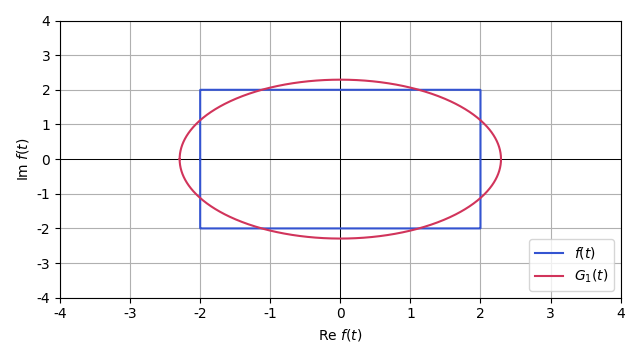
\includegraphics[width=\textwidth]{parametric_func/1.png}
        \caption{$n = 1$}
    \end{minipage}\hfill
    \begin{minipage}{0.5\textwidth}
        \centering 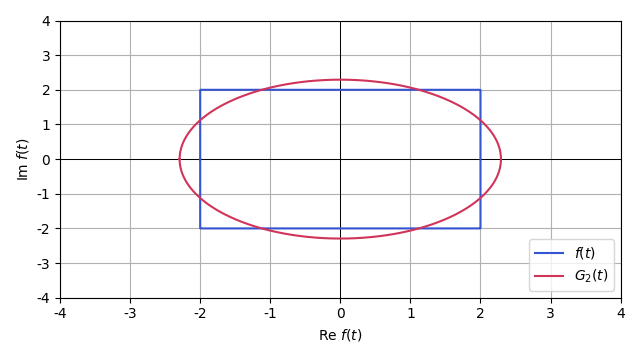
\includegraphics[width=\textwidth]{parametric_func/2.png}
        \caption{$n = 2$}
    \end{minipage}\\[2em]
    \begin{minipage}{0.5\textwidth}
        \centering 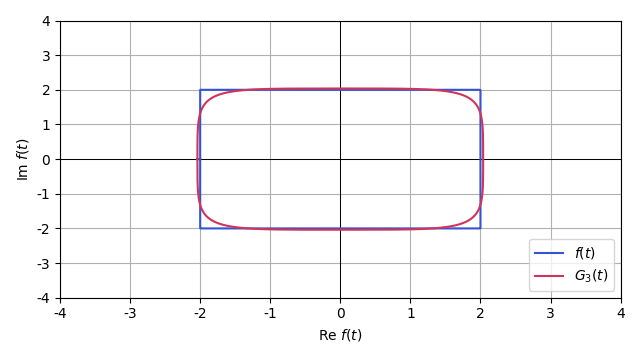
\includegraphics[width=\textwidth]{parametric_func/3.png}
        \caption{$n = 3$}
    \end{minipage}\hfill
    \begin{minipage}{0.5\textwidth}
        \centering 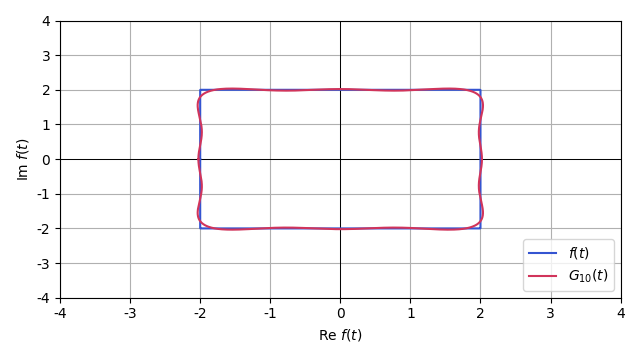
\includegraphics[width=\textwidth]{parametric_func/10.png}
        \caption{$n = 10$}
    \end{minipage}
\end{figure}\noindent
Начиная с первых значений, вокруг квадрата формируется круг, который становится с увеличением гармоник всё больше похож на квадрат. Мы убедимся в этом ещё раз, построив уже другие графики, где на абсциссе отложим t, а по ординате отложим сначала вещественные части $f(t)$ и $G_n(t)$, а затем мнимые части этих же функций.
\begin{figure}[H]
    \begin{minipage}{0.5\textwidth}
        \centering 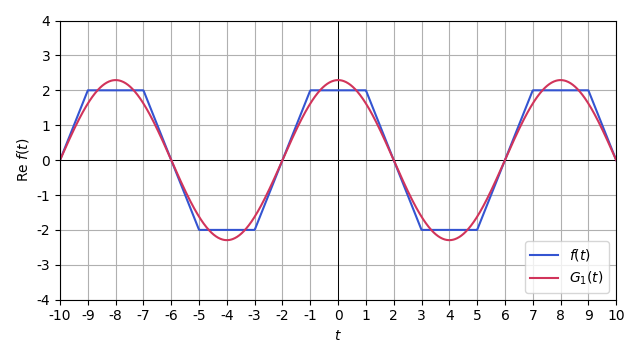
\includegraphics[width=\textwidth]{parametric_func/Re1.png}
        \caption{$Re\quad n = 1$}
    \end{minipage}\hfill
    \begin{minipage}{0.5\textwidth}
        \centering 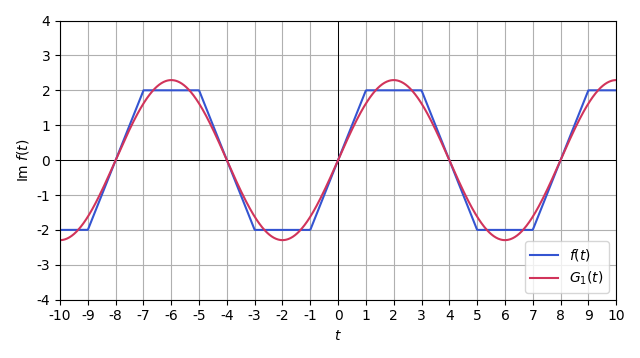
\includegraphics[width=\textwidth]{parametric_func/Im1.png}
        \caption{$Im\quad n = 1$}
    \end{minipage}
\end{figure}
\begin{figure}[H]
    \begin{minipage}{0.5\textwidth}
        \centering 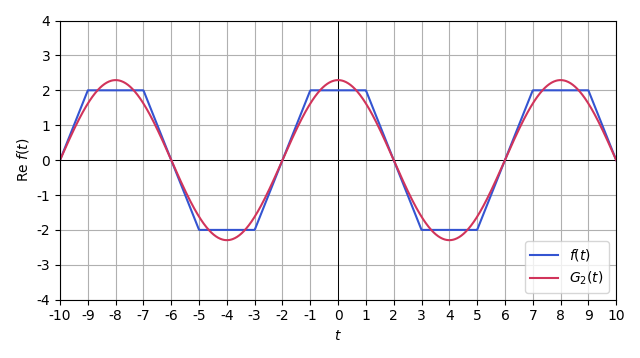
\includegraphics[width=\textwidth]{parametric_func/Re2.png}
        \caption{$Re\quad n = 2$}
    \end{minipage}\hfill
    \begin{minipage}{0.5\textwidth}
        \centering 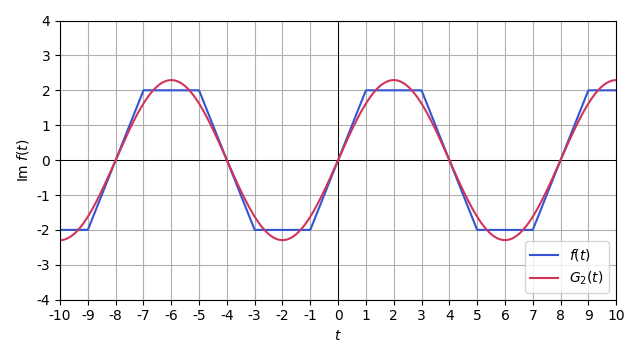
\includegraphics[width=\textwidth]{parametric_func/Im2.png}
        \caption{$Im\quad n = 2$}
    \end{minipage}\\[2em]
    \begin{minipage}{0.5\textwidth}
        \centering 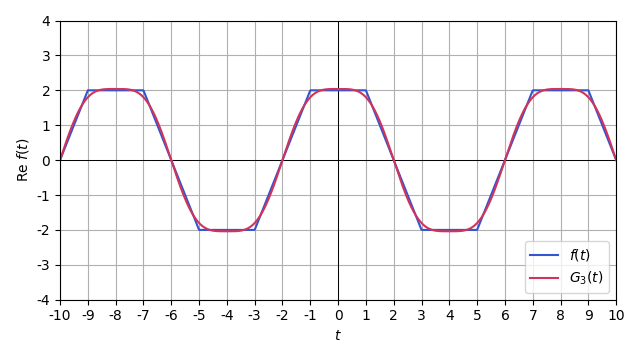
\includegraphics[width=\textwidth]{parametric_func/Re3.png}
        \caption{$Re\quad n = 3$}
    \end{minipage}\hfill
    \begin{minipage}{0.5\textwidth}
        \centering 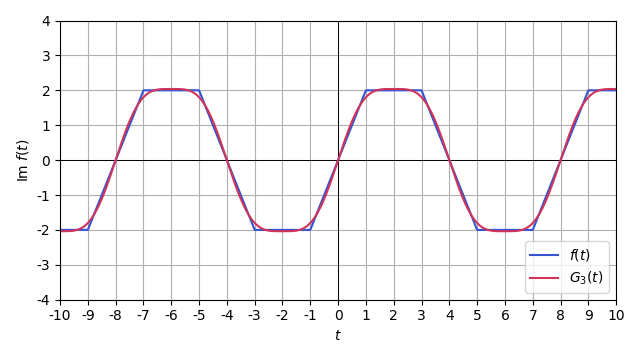
\includegraphics[width=\textwidth]{parametric_func/Im3.png}
        \caption{$Im\quad n = 3$}
    \end{minipage}\\[2em]
    \begin{minipage}{0.5\textwidth}
        \centering 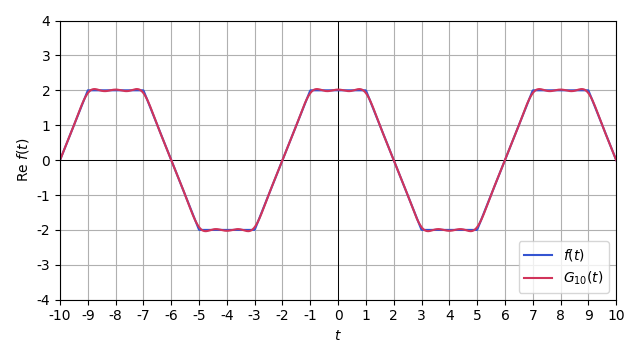
\includegraphics[width=\textwidth]{parametric_func/Re10.png}
        \caption{$Re\quad n = 10$}
    \end{minipage}\hfill
    \begin{minipage}{0.5\textwidth}
        \centering 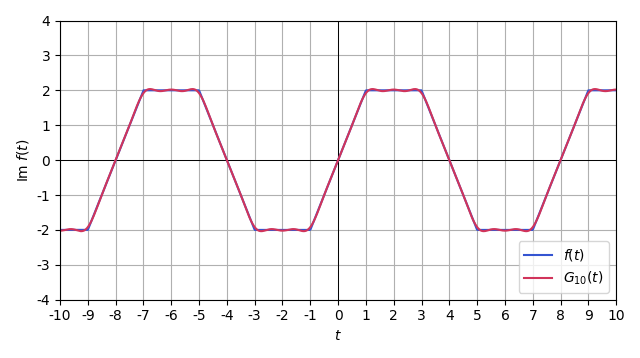
\includegraphics[width=\textwidth]{parametric_func/Im10.png}
        \caption{$Im\quad n = 10$}
    \end{minipage}
\end{figure}\noindent
Действительно, по графикам мы приходим к выводу, что $G_n(t)$ аппроксимирует исходную параметрическую комплекснозначную функцию $f(t)$, как в её действительной части, так и в мнимой.\\[0.5em]
Чтобы убедиться в том, что при $n = 10$ ряд Фурье очень точен к функции $f(t)$, проверим равенство Парсеваля при этом же количестве коэффициентов и при $n = 1$ --- так мы увидим разницу.\\
\begin{minipage}{0.48\textwidth}
\begin{lstlisting}[caption={Равенство Парасеваля при $n=1$}]
Parseval deviation:
| |f|^2 - sum(|a_i|^2 + |b_i|^2) | = 0.42457
| |f|^2 - sum(|c_i|^2) |           = 0.42457
\end{lstlisting}
\end{minipage}\hfill
\begin{minipage}{0.49\textwidth}
\begin{lstlisting}[caption={Равенство Парасеваля при $n=10$}, numbers=none]
Parseval deviation:
| |f|^2 - sum(|a_i|^2 + |b_i|^2) | = 0.00146
| |f|^2 - sum(|c_i|^2) |           = 0.00146
\end{lstlisting}
\end{minipage}
Мы наблюдаем, что отклонение в равенстве Парсеваля с увеличением количества коэффициентов стремится к нулю. Это означает, что ряд Фурье действительно приближается к функции $f(t)$ всё лучше и лучше.
\addsection{Подводим выводы, подытоживаем итоги}
В ходе выполнения лабораторной работы мы научились находить коэффициенты Фурье для различных функций и выяснили, что ряд Фурье может раскладываться как тригонометрически, так и комплексно.\\[0.5em]
Также пришли к выводу, что ряд Фурье раскладывается по разному в зависимости от чётности функции, и в нём могут отсутствовать как косинусы, если функция нечётная, так и синусы, если функция чётная, но в противном случае и в общем виде ряд Фурье раскладывается и по косинусам, и по синусам.\\[0.5em]
Мы убедились в том, что с увеличением количества членов ряда Фурье ряд первоклассно аппроксимирует исходную функцию --- это подтверждается как графически (мы наблюдали множество графиков, где с ростом количества суммируемых членов ряда Фурье наблюдалась всё лучшая и лучшая аппроксимация этим рядом функции), так и аналитически с помощью равенства Парсеваля, который говорит нам, что квадрат нормы исходной функции равен сумме квадратов модулей всех коэффициентов ряда Фурье (с ростом количества коэффициентов отклонение от квадрата нормы функции в равенстве Парсеваля стремится к нулю).\\[0.5em]
\end{document}